\documentclass{article}
\title{ECE 341 -- Homework 1}
\usepackage{graphicx}
\usepackage{float}
\usepackage{pdfpages}
\usepackage{fancyhdr}
\usepackage{enumitem}
\usepackage{pdfpages}
\usepackage{amsmath}
\usepackage{amssymb}
\pagestyle{fancy}
\fancyhf{}
\fancyhead[L]{Gianni Avilan-Losee}
\fancyhead[C]{ECE 341}
\fancyhead[R]{Homework 1}
\fancyfoot[C]{\thepage}
\usepackage{microtype}
\usepackage{textcomp, gensymb}
\author{Gianni Avilan-Losee}
\begin{document}

\includepdf{homework-1_cover-page.pdf}
\begin{enumerate}[label=\thesubsubsection]
\setcounter{section}{1}
\setcounter{subsection}{1}
\setcounter{subsubsection}{1}
		\item
		\begin{enumerate}[label=\alph*)]
			\item \(x_a(t)\)'s energy is given by \[
			 E_a = \int_{-\infty}^{\infty}|x(t)|^2dt = \int_{0}^{2}1dt + \int_{2}^{3}1dt = 2 + 1 = 3.
			\] 
		  \item \(x_b(t) = -x_a(t)\), and its energy is given by \[
		    E_b = \int_{0}^{2}1dt + \int_{2}^{3}1dt = 3.
			\]  
		  \item \(x_c(t) = x_a(t-3)\), and its energy is given by \[
		    E_c = \int_{3}^{5}1dt + \int_{5}^{6}1dt = 3.
		  \]
		  \item \(x_d(t) = 2x_a(t)\), and its energy is given by \[
        E_d = 4(\int_{0}^{2}1dt + \int_{2}^{3}1dt) = 4(3) = 12.	
		  \]
		\end{enumerate}
		Since a signals energy is based off the absolute value of the signal, \(|x(t)|\), sign changes have no effect on the energy, since \(|-x(t)| = x(t)\). Additionally, since energy is the sum of all values of \(t \in (-\infty, \infty)\), time-shifting has no effect on the energy. Finally, since energy is based off the square \(|x(t)|^2\) of the given signal, doubling the signal will increase its energy by a factor of \(2^2 = 4\), and multiplying the signal by \(k\) will increase its energy by a factor of \(k^2\). In other words, \[
		  E_{kx(t)} = k^2E_{x(t)}.
		\] 
		\setcounter{subsubsection}{4}
	\item The signal shown in Fig. P1.1-4 is periodic with a period of \(T=4\), and thus has an energy of 0; therefore, power is a more meaningful measure of the signal's energy. Its power is given by \[
			P_x = \frac{1}{4}\int_{-2}^{2}|x(t)|^{2}dt = \frac{1}{4}\int_{-2}^{2}t^6dt \approx 9.14.
	\] 
	The RMS value is given by the square root of the power, \[
		P_{rms} = \sqrt{9.14} \approx 3.02.
	\]
	\begin{enumerate}[label=\alph*)]
		\item The power of \(x(t) = -x(t) = -t^3\) is found as \[
				P_{-x} = \frac{1}{4}\int_{-2}^{2}|-t^3|^2dt \approx 9.14, 
		\]
		with an RMS value of \(\sqrt{9.14} \approx 3.02.\) 
	  \item The power of \(x(t) = 2x(t) = 2t^3\) is found as \[
				P_{2x} = \frac{1}{4}\int_{-2}^{2}|2t^3|^2dt = \frac{1}{4}\int_{-2}^{2}4t^6dt \approx 36.57, 
	  \]
		with an RMS value of \(\sqrt{36.57} \approx 6.05.\)
	  \item The power of \(x(t) = cx(t) = ct^3\) is found as \[
				P_{cx} = \frac{1}{4}\int_{-2}^{2}|ct^3|^2dt = \frac{1}{4}\int_{-2}^{2}c^2t^6dt = c^2(9.14),
	  \] with an RMS value of \(\sqrt{c^2(9.14)} = c(3.02).\)
	\end{enumerate}
	\setcounter{subsection}{2}
	\setcounter{subsubsection}{1}
	\item
    The given signal, along with its permutations, are labeled on the y-axis and shown below (graphs were created in MATLAB from scratch):
		\begin{figure}[H]
		  \centering
			\makebox[\textwidth]{%
		  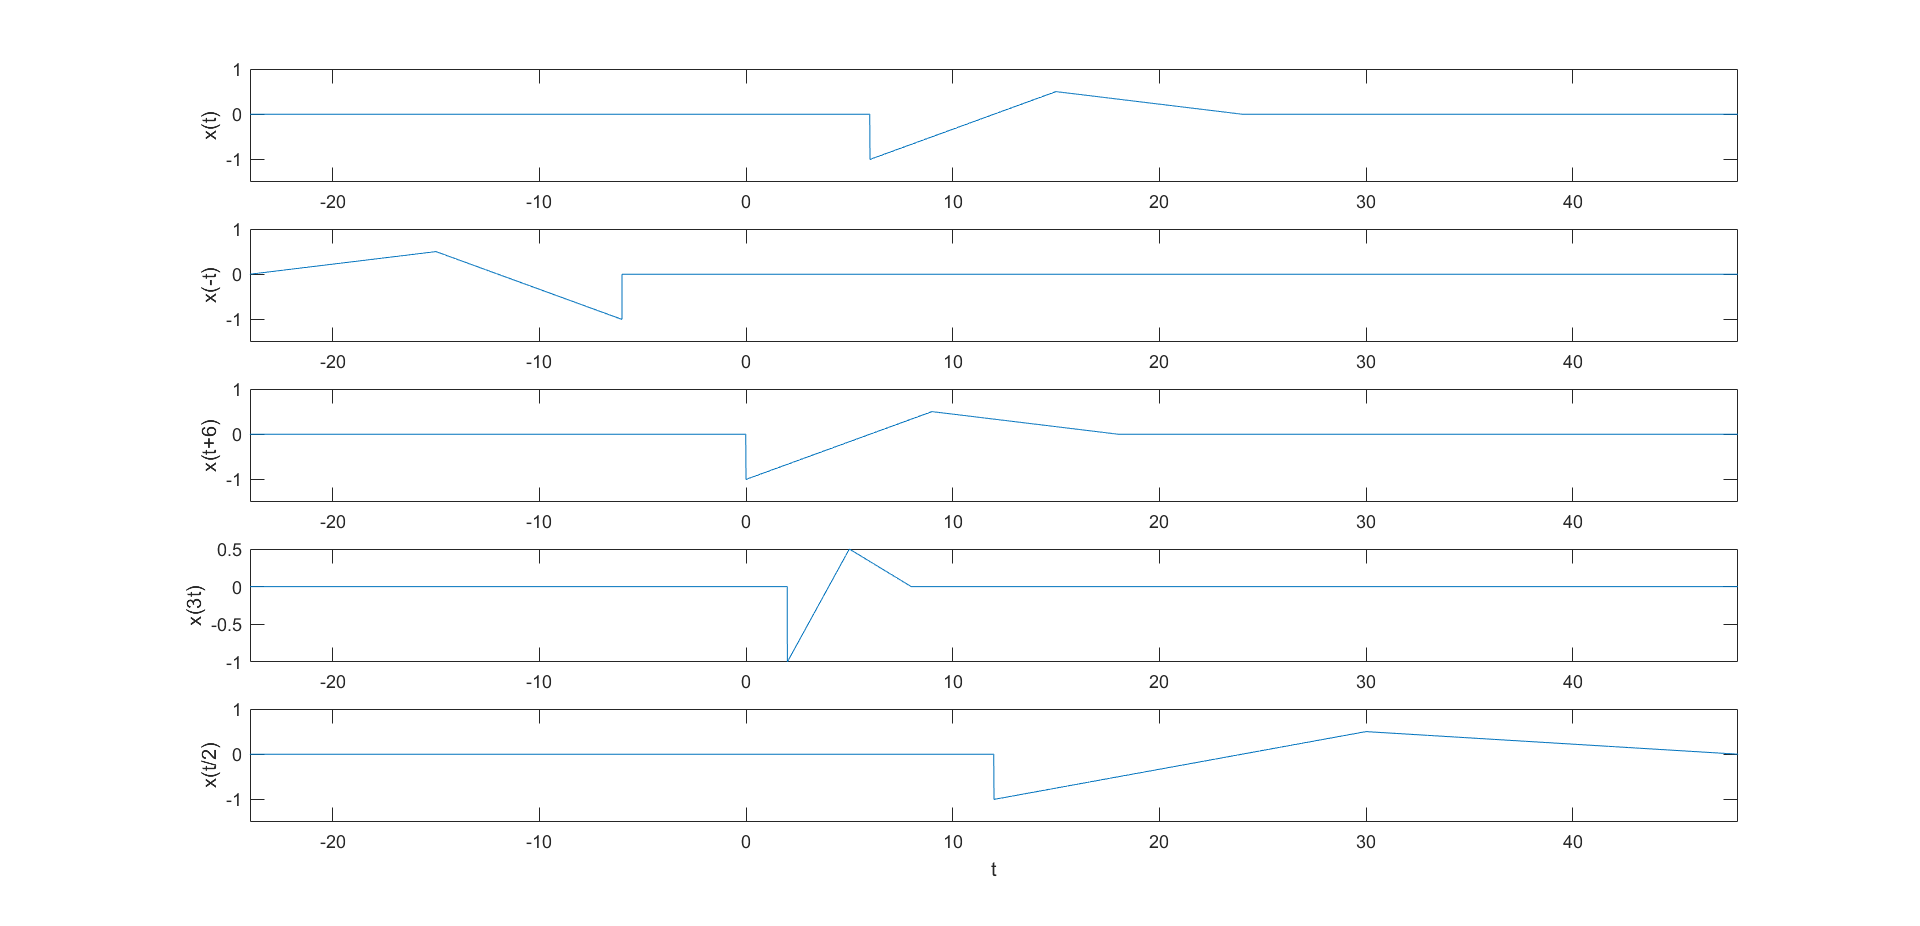
\includegraphics[width=1.5\textwidth]{homework-1_fig-1.png}%
		}
		  \caption{\(x(t)\) and its permutations}
		  \label{fig:x(t) and permutations}
		\end{figure}
		\setcounter{subsection}{4}
		\setcounter{subsubsection}{2}
  \item
		\begin{enumerate}[label=\alph*)]
			\item \(x_{1}(t) = (4t+4)(u(t+1) - u(t)) + (-2t+4)(u(t)-u(t-2)).\)
			\item \(x_{2}(t) = t^2(u(t)-u(t-2)) + (2t- 8)(u(t-2) - u(t-4)).\) 
		\end{enumerate}
		\setcounter{subsection}{5}
		\setcounter{subsubsection}{4}
	\item 
		\begin{enumerate}[label=\alph*)]
			\item The product of an even and an odd function equals an odd function, \(x_e(t)x_o(t) = x_o(t)\), and the integral of an odd function over any symmetric bound \((-a,a)\)is equal to 0, as the negative and positive components cancel out. Mathematically, \[
        \int_{-\frac{a}{2}}^{0}x_o(t)dt + \int_{0}^{\frac{a}{2}}x_o(t)dt = 0.
      \]
			Therefore, the integral of the product \(x_o(t)x_e(t) = x_o(t)\) is always equal to 0 on the interval \((-\infty, \infty)\).
			\item Since the integrals of odd functions on symmetric bounds, as mentioned above, always evaulate to 0, and all functions \(x(t)\) are the sum of an even and odd component \(x_o(t) + x_e(t)\), we can express the integral of any function \(x(t)\) on the bound \((-\infty, \infty)\) as \[
			  \int_{-\infty}^{\infty}x(t)dt = \int_{-\infty}^{\infty}x_o(t) + \int_{-\infty}^{\infty}x_e(t)dt = 0 + \int_{-\infty}^{\infty}x_e(t)dt.
			\]
		\end{enumerate}
		\setcounter{subsection}{7}
    \setcounter{subsubsection}{2}
		\item
			For a time-invariant system \(y(t) = x(t)\), supposing \(x_1(t) = x(t)\) and \(y_1(t) = y(t)\), time shifting the input such that \(x_2(t) = x_1(t-t_0)\) should result in an equivalent shift of \(y_2(t) = y_1(t-t_0)\), so that \(y_1(t) = x_1(t)\) and \(y_2(t) = x_2(t).\) If this is not the case, the system is considered time-variant.
		\begin{enumerate}[label=\alph*)]
			\item
				Given \(x_1(t) = x(t-2)\), \(x_2(t) = x_1(t-t_0) = x(t-t_0-2)\). Then, shifting the output by the same time delay, \(y_2(t) = y_1(t-t_0) = x_1(t-t_0-2)\). 
				
				\(y_2(t) = x(t-t_0-2) = x_2(t)\), proving that the system is time invariant.
			 \item
				 Given \(x_1(t) = x(-t)\), \(x_2(t) = x_1(t-t_0) = x(-t-t_0)\). Then, shifting the output by the same time delay, \(y_2(t) = y_1(t-t_0) = x(-(t-t_0)) = x(-t+t_0).\) . 

				 \(y_2(t) = x(-t+t_0) \neq x(-t-t_0) = x_2(t)\), proving that the system is time variant.
			 \item 
				 Given \(x_1(t) = x(at)\), \(x_2(t) = x_1(t-t_0) = x(at-t_0)\). Then, shifting the output by the same time delay, \(y_2(t) = y_1(t-t_0) = x(a(t - t_0)) = x(at-at_0)\).  

				 \(y_2(t) = x(at-at_0) \neq x(at-t_0) = x_2(t)\), proving that the system is time variant.
			 \item 
				 Given \(x_1(t) = tx(t-2)\), \(x_2 = x_1(t-t_0) = tx(t-t_0-2)\). Then, shifting the output by the same time delay, \(y_2(t) = y_1(t-t_0) = (t-t_0)x(t-t_0-2)\). 

				 \(y_2(t) = (t-t_0)x(t-t_0-2) \neq tx(t-t_0-2) = x_2(t)\), proving that the system is time variant.

				 \item
					Given \(y(t) = \int_{-5}^{5}x(\tau)d\tau\), a simple counterexample may be used to show that the system is time variant.

					Assuming that \(x_1(t) = \delta(t)\), then \[
					  y_1(t) = \int_{-5}^{5}\delta(\tau)d\tau = 1.
					\]
					Assuming that \(x_2(t) = \delta(t-10)\), then \[
					  y_2(t) = \int_{-5}^{5}\delta(\tau)d\tau = 0.
					\]
					Since the output of \(y_1(t) = 1\) is a constant (does not depend on t), in a time-invariant system, we would expect \(y_2(t) = y(t-10) = 1\). However, \(y_2(t) = 1 \neq 0 = x_2(t)\), and so the system is time variant.
				 \item 
					 Given \(x_1 = (\frac{dx(t)}{dt})^2\), \(x_2(t) = x_1(t-t_0) = (\frac{dx(t-t_0)}{dt})^2\). Then, shifting the output by the same amount, \(y_2(t) = y_1(t-t_0) = (\frac{dx(t-t_0)}{d(t-t_0)})^2\). Note that \(dt\) and \(d(t-t_0)\) have the same value, as they are infintesimal quantites, and thus we can say \(dt = d(t-t_0)\).
					 Therefore, \(y_2(t) = \frac{dx(t-t_0)}{dt} = x_2(t)\), proving the system is time invariant. 
		\end{enumerate}
		\setcounter{subsubsection}{15}
		\item
	  \begin{enumerate}[label=\alph*)]
			\item For \(y(t) = x(t-2)\), the system is causal, since \(t > t-2\) for all values of \(t\), and therefore \(y(t)\) depends on future values of \(t\) regardless of the input.
			\item For \(y(t) = x(-t)\), the system is noncausal, since, for negative values of \(t = -t\), \(-t < -(-t) = t\), making \(y(t)\) dependent on a future value of \(t\) for \(t < 0\). 
			\item For \(y(t) = x(at)\), \(a > 1\), the system is noncausal, since \(t \leq at\) for all values of \(t\) and \(a > 1\), making \(y(t)\) dependent on future values of \(t\) for \(a\neq1\).      
			\item For \(y(t) = x(at)\), \(a<t\), the system is noncausal, since \(t < at\) for all values of \(t < 0\) and \(a<1\), making the system dependent on future values of \(t\) for \(t < 0\).
		\end{enumerate}
\end{enumerate}
\end{document}
